\documentclass[10pt, conference]{IEEEtran}
\IEEEoverridecommandlockouts
% The preceding line is only needed to identify funding in the first footnote. If that is unneeded, please comment it out.
\usepackage{cite}
\usepackage{amsmath,amssymb,amsfonts}
\usepackage{algorithm}
% \usepackage{algorithmic}
\usepackage{algpseudocode}
\usepackage{graphicx}
\usepackage{textcomp}
\usepackage{xcolor}
\usepackage{bm}
\usepackage[acronym]{glossaries}
\def\BibTeX{{\rm B\kern-.05em{\sc i\kern-.025em b}\kern-.08em
    T\kern-.1667em\lower.7ex\hbox{E}\kern-.125emX}}


\makeglossaries

\newacronym{cart}{CART}{classification and regression trees}
\newacronym{eda}{EDA}{exploratory data analysis}
\newacronym{id3}{ID3}{iterative dichotomiser 3}
\newacronym{knn}{KNN}{k-nearest neighbours}
\newacronym{mar}{MAR}{missing at random}
\newacronym{mcar}{MCAR}{missing completely at random}
\newacronym{ni}{NI}{nonignorable}


\begin{document}

\title{Assignment 1\\
% {\footnotesize \textsuperscript{*}Note: Sub-titles are not captured in Xplore and
% should not be used}
% \thanks{Identify applicable funding agency here. If none, delete this.}
}

\author{\IEEEauthorblockN{Andre van der Merwe}
% \IEEEauthorblockA{\textit{dept. name of organization (of Aff.)} \\
% \textit{name of organization (of Aff.)}\\
% City, Country \\
% email address or ORCID}
}

\maketitle

\begin{abstract}
    
\end{abstract}

\section{Introduction}



\section{Background}

This section presents background information on \\ \acrlong{eda} and techniques used to clean and transform data
for analysis or to construct models. Additionally, information on the C4.5 decision tree and k-nearest neighbours
classification models.

\subsection{Exploratory Data Analysis}\label{EDA}

Exploratory data analysis \acrshort{eda} first introduced by John Tukey in 1977 \cite{EDA_ref}. Tukey
emphasised that there are three key strategies in data analysis, namely:
\begin{itemize}
    \item Grapical presentation: the use of visual tools, such as plots, to explore, analyse and understand data.
    \item Flexibility in viewpoint and facilities: encourages creative and diverse approaches to analyse data
          that allows for dynamic perspective and adaptive tools.
    \item Search for parsemony and simplicity: To find simple and clear explanations in the data while
          unnecessary complexity is avoided.
\end{itemize}

\subsubsection{Data Quality Issues}

\paragraph{Missing values}

The absence of data in a dataset where a value should be present is known as a missing value. There are
three types of missing values, namely \acrfull{mar}, \acrfull{mcar} and \acrfull{ni} missing values \cite{Missing_ref}.

\acrshort{mcar} refers to a situation where missing values are distributed randomly throughout the dataset, independent
of both observed and unobserved data. Under \acrshort{mcar}, modern methods such as missing value imputation can be
used and still produce unbiased estimates, though some uncertainty is introduced. When modern methods are used
to handel \acrshort{mcar} missing values, the statistical power reduces compared to complete data.

A missing value is \acrshort{mar} if the likelihood of the missing data on the variable is unrelated to the value of
that variable itself, once other variables are taken into account. These other features help explain why data may
be missing and is known as mechanisms. Some common mechanisms include factors like education, income or age.
The \acrshort{mar} assumption holds if the pattern of missingness is random when explained by the mechanisms.

If data is missing in a systematic way and can neither be classified as \acrshort{mar} or \acrshort{mcar}, then
is the missing value classified as \acrshort{ni}. To model this type of data is complex.

There are three ways to deal with these missing values. The first option explored is to use machine learning
algorithms that is robust to missing values. The second option is to remove the instances that contains the
missing values. This option does run the risk of valuable information that may be lossed. The third option
is to impute the missing values.

When a missing value is imputed from a categorical feature, the most frequently occuring value, known as the mode,
is commonly used. When a numerical feature is imputed, the median is typically used when the data contains outliers
and the mean is used when the data contains no outliers. 

\paragraph{Outliers}

When one or more variables, of an instance in the data set, have values that significantly differ from the overall distribution
of the data, it is known as an outlier. There are two types of outliers, namely invalid outliers that is data points included
in the data set due to errors, and valid outliers that is correct values that are legitimately different from the rest
of the data.

There are three techniques to cope with outliers. The first technique is to remove the outliers using statistical
techniques. The second technique is to keep the outliers and apply robust estimators that are less sensitive to the
influence of the outliers. Alternatively, clipping can be performed to the outliers to limit the range of the outliers
or to impute a value to replace the outlier with. The third technique is to remove the outliers directly within the
machine learning process by the use of algorithms designed to be robust to outliers.

One approach to perform outlier detection 

\paragraph{Noise}

\paragraph{Imbalanced class data}

\subsubsection{Data Preparation}

\paragraph{Data type transformations}

\paragraph{Feature selection}

\paragraph{Normalisation}

Normalisation or scaling of input features is required for some machine learning algorithms. Normalisation
is typically required if the ranges of values for different input features differ in order of magnitudes 
and where the algorithm makes use of a distance based metric to generate classification
models. Normalisation is also used when the minimum and maximum values are not known, to
reduce the effect of outliers or to transform a range of values to a different range of values.

\subsection{K-Nearest Neighbours}\label{KNN}

The \acrfull{knn} algorithm was first propsed by Evelyn Fix and Joseph Hodges in 1951 \cite{KNN_ref}
in a technical report that was never published. The report contained pioneering work on nonparametric
discriminant analysis and probability density estimation and laid the foundational principles for
the \acrshort{knn} algorithm.

\acrshort{knn} is a type of instance-based learning that does not build a model based on the training
dataset. Instead, \acrshort{knn} computes the distance between the instances in the test set and all
of the instances in the training set to identify the nearest neighbours for each entry in the test set.
\acrshort{knn} relies heavily on the distance metric in order to identify the instances in the training
set closest to each of the test instances. The distance metric plays a crucial role in order to determine
the similarity between data points, that directly influences the performance and accuracy of the algorithm.
The most common distance metrics used in the \acrshort{knn} algorithm is the:
\begin{itemize}
    \item Euclidean distance metric
    \item Manhattan distance metric
    \item Minkowski distance metric
\end{itemize}

The Euclidian distance metric equation is defined as follows:
\begin{equation}
    d(\boldsymbol{\textbf{x}}_1, \boldsymbol{\textbf{x}}_2) = \sqrt{\sum_{n=1}^{N}(x_{1n} - x_{2n})^2} \label{euclidian}
\end{equation}
The Manhattan distance metric equation is defined as follows:
\begin{equation}
    d(\boldsymbol{\textbf{x}}_1, \boldsymbol{\textbf{x}}_2) = \sum_{n=1}^{N} \left| x_{1n} - x_{2n} \right| \label{manhattan}
\end{equation}
The Minkowski distance metric equation is defined as follows:
\begin{equation}
    d(\boldsymbol{\textbf{x}}_1, \boldsymbol{\textbf{x}}_2) = \left(\sum_{n=1}^{N} \left| x_{1n} - x_{2n} \right|^p\right)^\frac{1}{p} \label{minkowski}
\end{equation}
where $\boldsymbol{\textbf{x}}_1$ and $\boldsymbol{\textbf{x}}_2$ is a vector containing all the of the features of two
distinct instances in a dataset, $d(\boldsymbol{\textbf{x}}_1, \boldsymbol{\textbf{x}}_2)$ is the distance between the two
vectors $\boldsymbol{\textbf{x}}_1$ and $\boldsymbol{\textbf{x}}_2$, $N$ denotes the dimension of the vectors 
$\boldsymbol{\textbf{x}}_1$ and $\boldsymbol{\textbf{x}}_2$ or equivalently the total number of features and $x_{1n}$ and
$x_{2n}$ is the value of the $n$-th feature of the two distinct feature vectors $\boldsymbol{\textbf{x}}_1$ and
$\boldsymbol{\textbf{x}}_2$ respectively.

After the distances between the instance from the test set is calculated against all of the instances in the training set,
a distance vector $\boldsymbol{\textbf{d}}$ is obtained. The distance vector is then sorted from smallest to largest distances
and the first $k$ distances is chosen from $\boldsymbol{\textbf{d}}$. The process to classify an unseen instance,
$\boldsymbol{\textbf{x}}$, on $k$ of the instances of the training set $D$ is described by Algorithm \ref{alg:KNN_algorithm}.
\begin{algorithm}
\caption{k-Nearest Neighbors (kNN)}
\label{alg:KNN_algorithm}
\begin{algorithmic}[1]
    \Function{kNN}{$D$, $\boldsymbol{\textbf{x}}$, $k$}
        \ForAll{$\boldsymbol{\textbf{x}}_i \in D$}
            \State $\boldsymbol{\textbf{d}}$ = \Call{distance}{$\boldsymbol{\textbf{x}}_i, \boldsymbol{\textbf{x}}$}
        \EndFor
        \State \Call{sort}{$\boldsymbol{\textbf{d}}$}
        \State $S$ = set of $k$ patterns in $D$ closest to $\boldsymbol{\textbf{x}}$
        \State Return class as majority class in $S$
    \EndFunction
\end{algorithmic}
\end{algorithm}

\subsection{C4.5 Decision Trees}\label{CT}

The first implementation of a decision tree algorithm was introduced by Leo Brieman \textit{et al} in 1984 and
is know as \acrfull{cart} \cite{CART_ref}. In 1986 Ross Quinlan implemented the \acrfull{id3} decision tree
algorithm, which is able to cope with noise and missing values in the data \cite{ID3_ref}. In 1993 Ross Quinlan
introduced the C4.5 decision tree algorithm, which is able to handle continuous features, imbalanced classes and
introduced post-pruning \cite{C4.5_ref}.

C4.5 generates a classification tree model that consists of:
\begin{itemize}
    \item Leaf nodes that indicates different discrete classes
    \item Decision nodes that represent tests on a feature and leads to further branches in the tree.
\end{itemize}
C4.5 is induced to overfit the training data, thus the tree classifier completely separates the classes of the
training data and leads to poor generalisation on usneen data as well as outliers and noise will be in the leaves of
the tree. In order to overcome these issues, C4.5 introduced post-pruning. 

C4.5 uses entropy as a measure of impurity in a dataset with respect to the target feature. The entropy of a
dataset will be 0, if all of the classes in the dataset has the same labels. If the frequency of the
classes are all equal, then will the entropy of the dataset be equal to 1. The test on an input feature
that minimises the impurity of a dataset, or equivalently maximises the information gain, is selected as the
best possible feature to split on. The equation to calculate the entropy of a dataset is as follows:
\begin{equation}
    H(D)=-\sum_{i=1}^{M} p(y_m)log_M (p(y_m))\label{entropy}
\end{equation}
and:
\begin{equation}
    p(y_m) = \frac{freq(y_m,D)}{\left\lvert D \right\rvert }\label{class_prob} 
\end{equation}
where $D$ represents the dataset, $y_m$ is the $m$-th class, $M$ is the total number of distinct classes in the
dataset, $p(y_m)$ is the probability of a class $y_m$ occuring in $D$ and where $freq(Y_m,D)$ is the number of
times class $y_m$ occurs in D.

The equation used to calculate the entropy due to the split, follows as:
\begin{equation}
    H_x(D) = \sum_{o=1}^{O} p_o H(D_o)\label{entropy_x}
\end{equation}
and:
\begin{equation}
    p_o = \frac{\left\lvert D_o \right\rvert}{\left\lvert D \right\rvert}\label{o_prob}
\end{equation}
where $x$ is the input variable used to split $D$, $O$ is the number of outcomes for $x$, $H(D_o)$ is the copnditional entropy of dataset
$D_o$ with reference to the class distribution and where $p_o$ is the probability of outcome $o$.

The equation used to calculate the information gain if $D$ is partitioned on $x$, follows as:
\begin{equation}
    gain(x) = H(D) - H_x(D)\label{info_gain}
\end{equation}
The information gain calculation \eqref{info_gain} favours input features with many outcomes and introduces bias as the tree
creates multiple branches, one for each unique value. The solution to the bias is to normalise the information gain with entropy
with respect to test outcomes. The equation for the gain ratio is as follows:
\begin{equation}
    gainRatio(x) = (1-F)\frac{gain(x)}{splitInfo(x)}\label{gainRatio}
\end{equation}
and:
\begin{equation}
    splitInfo(x) = -\sum_{o=1}^{O}p_o log_O(p_o)\label{splitInfo}
\end{equation}
where $F$ is the fraction of patterns in $D$ for which the value of $x$ is missing.
The objective of the tree is to select $x$ that maximise the gain ratio \eqref{gainRatio}

In order to handel numerical continuous features, C4.5 first sorts the number of unique values, denoted by $I$,
found in the numeric input feature $x$ to create the sequence, $(v_1,v_2,...,v_I)$ ordered from smallest to largest.
C4.5 performs $I$-1 splits between $v_i$ and $v_{i+1}$ and for each of these splits the information gain is calculated \eqref{gainRatio}.
The split with the highest calculated information gain will be chosen and the threshold to split the tree on is calculated as follows:
\begin{equation}
    \epsilon = \frac{v_i + v_{i+1}}{2}\label{numeric}
\end{equation}
where $\epsilon$ is the threshold to split the tree on. C4.5 then generates two decision nodes with test $x < \epsilon$ and $x >= \epsilon$.

C4.5 partitions the dataset $D$ in the absence of missing values as follows: 
\begin{equation}
    w_j(D_o) = 1, w_j(D_q)=0, \forall q \neq o \label{no_missing}
\end{equation}
where each pattern $j$ in $D$ belongs to subset $D_o$ with weight $w_i(D_o)$, provided that pattern $j$ no missing value for the input
feature $x$. If pattern $j$ has a missing value for feature $x$, it is assigned to all outcomes with a weight given by:
\begin{equation}
    w_j(D_o) = w_j(D)p_o \label{with_missing}
\end{equation}
where the probability of the outcome is now calculated as follows:
\begin{equation}
    p_o = \frac{\Sigma_{x_j \epsilon D \text{ with outcome } _o} w_j(D)}{\Sigma_{x_j \epsilon D \text{ with any known outcome}} w_j(D)}
\end{equation}

To determine the optimal input feature $x$ to split the data on, the process follows these steps:
\begin{itemize}
    \item Calculate the entropy of the current data set, $H(D)$ \eqref{entropy}
    \item Compute the conditional entropy for each input feature $x$, $H_x(D)$ \eqref{entropy_x}
    \item Calculate the information gain for each feature if $D$ would be split on $x$ \eqref{info_gain}
    \item Using the calculated information gain, calculate the gain ratio \eqref{gainRatio}
    \item Select the feature with the highest gain ratio and split $D$ into $O$ subsets
    \item Repeat the process on each subset until the tree has been induced to completely separate the classes
\end{itemize}

Algorithm \ref{alg:CTI_algorithm} describes the process to fully induce the decision tree. 
\begin{algorithm}
    \caption{Classification Tree Induction}
    \label{alg:CTI_algorithm}
    \begin{algorithmic}[1]
        \Function{InduceTree}{$D$}
            \If{$\left\lvert D \right\rvert$ = 0}
                \State Return leaf with default class
            \EndIf
            
            \If{$\left\lvert D \right\rvert$ $>$ 0 and $\forall \boldsymbol{\textbf{x}} \in D$ the class is the same, i.e. $y_m$}
                \State Return leaf with class label $y_m$, containing $D$
            \EndIf{}

            \State Select a test based on a single input variable
            \State Split $D$ into $D_1$,$D_2$,...,$D_o$, where $O$ is the number of outcomes
            \For{$o$ = 1 to $O$}
                \State \Call{InduceTree}{$D_o$}
            \EndFor
        \EndFunction
    \end{algorithmic}
\end{algorithm}

\section{Methodology}

\subsection{Classification Tree}

C4.5 replaces the tests in the deepest level of the tree with leaf nodes,
where the prediction of the leaf node is the class that occurs the most in the new subset.
A validation set is used to test the generalisation performance of unseen data and if the generalisation performance
increases, the tree prunes away the decision node and replaces it with the leaf node. If the generalisation performance
does not improve, the decision node is then re-inserted into the tree. This process is repeated until no more decision
nodes are replaced. The tree is now robust to outliers and noise 


\section{Empirical Procedure}
\section{Research Results}
\section{Conclusion}
\begin{thebibliography}{00}
    \bibitem{Missing_ref} A. C. Acock "Working with missing values." In: Journal of Marriage and family (2005).
    \bibitem{CART_ref} L. Breiman, J. Friedman, R. A. Olshen and C. J. Stone "Classification and Regression Trees." In: Routledge.  (1984).
    \bibitem{KNN_ref} M. C. Jones, B. W. Silverman “E. Fix and J.L. Hodges (1951): An Important Contribution to Nonparametric Discriminant Analysis and Density Estimation: Commentary on Fix and Hodges (1951).” In: International Statistical Review / Revue Internationale de Statistique, vol. 57, no. 3, (1989).
    \bibitem{ID3_ref} J. R. Quinlan "Induction of decision trees" In: Mach Learn 1 (1986).
    \bibitem{C4.5_ref} J. R. Quinlan "C4. 5: programs for machine learning." In: Elsevier, (1993).
    \bibitem{EDA_ref} J. W. Tukey. "Exploratory data analysis." In: Reading/Addison-Wesley (1977).
\end{thebibliography}


\printglossary[type=\acronymtype]

\clearpage

\begin{table}[h!]
    % \caption{\textbf{Continuous Features}}
    \caption{Continuous Features}
    \begin{center}
    \begin{tabular}{|c||c|c|c|c|c|c|c|c|c|c|}
        \hline
        \textbf{Features}&\textbf{Count}&\textbf{\% Miss.}&\textbf{Card.}&\textbf{Min.}&\textbf{$1^{st}$ Qrt.}&\textbf{Mean}&\textbf{Median}&\textbf{$3^{rd}$ Qrt.}&\textbf{Max}.&\textbf{Std Dev.}\\
        \hline
        %   	                    Count   % Miss     Card.    Min         1st Q       Mean          Median      3rd Q       Max         Std Dev
        \textbf{Area}               &13611  &0.0       &12011   &20420      &36328      &53048.284549 &44652      &61332      &254616     &29324.095717\\
        \textbf{Perimeter}          &13611  &0.0       &13351   &524.736    &703.5235   &855.283459   &794.941    &977.213    &1985.37    &214.289696\\
        \textbf{MajorAxisLength}    &13611  &0.0       &13543   &183.601165 &253.303633 &320.141867   &296.883367 &376.495012 &738.860153 &85.694186\\
        \textbf{MinorAxisLength}    &13611  &0.0       &13543   &122.512653 &175.848170	&202.270714   &192.431733 &217.031741 &460.198497 &44.970091\\
        \textbf{AspectRation}       &13611  &0.0       &13543   &1.024868   &1.432307   &1.583242     &1.551124   &1.707109	  &2.430306   &0.246678\\
        \textbf{Eccentricity}       &13611  &0.0       &13543   &0.218951   &0.715928   &0.750895     &0.764441	  &0.810466	  &0.911423   &0.092002\\
        \textbf{ConvexArea}         &13611  &0.0       &12066   &-30        &36714.5    &53765.692602 &45178      &62294      &263261     &29778.009358\\
        \textbf{EquivDiameter}      &13611  &0.0       &12012   &0.161417   &215.068003 &476.254106   &238.438026 &279.452162 &3014441    &25836.865632\\
        \textbf{Extent}             &13611  &0.044082  &13529   &0.555315   &0.718641   &0.749747     &0.759874   &0.786852	  &0.866195	  &0.049085\\
        \textbf{Solidity}           &13611  &0.0       &13526   &0.919246	&0.985670	&0.987143     &0.988283   &0.990013   &0.994677   &0.004660	\\
        \textbf{Roundness}          &13611  &0.0       &13543   &0.489618   &0.832096   &0.873282     &0.883157   &0.916869   &0.990685   &0.059520\\
        \textbf{Compactness}        &13611  &0.132246  &13525   &0.640577	&0.762577	&0.799886	  &0.801291	  &0.834270   &0.987303   &0.061684\\
        \textbf{ShapeFactor1}       &13611  &0.0       &13543   &0.002778   &0.005900   &0.006564	  &0.006645   &0.007271   &0.010451   &0.001128\\
        \textbf{ShapeFactor2}       &13611  &0.0       &13543   &0.000564	&0.001154	&0.001716	  &0.001694	  &0.002170   &0.003665   &0.000596\\
        \textbf{ShapeFactor3}       &13611  &0.0       &13543   &0.410339   &0.581359	&0.643590     &0.642044	  &0.696006	  &0.974767   &0.098996\\
        \textbf{ShapeFactor4}       &13611  &0.0       &13611   &0.695579	&1.614151	&2.368097	  &2.368757   &3.115695	  &3.966119   &0.871619\\
        \textbf{ShapeFactor5}       &13611  &0.0       &13543   &0.947687   &0.993703   &0.995063	  &0.996386	  &0.997883   &0.999733   &0.004366\\
        \textbf{ShapeFactor6}       &13611  &0.036735  &13606   &0.000466	&45.258826	&89.358603	  &88.76667   &134.273148 &178.985023 &51.838555\\
        \textbf{Sort order}         &13611  &0.0       &13611   &0.000089   &0.248187   &0.500271     &0.50381    &0.750096   &0.999985   &0.287926\\

        \hline
    \end{tabular}
    \label{continuous features}
    \end{center}
\end{table}

\begin{table}[h!]
    % \caption{\textbf{Continuous Features}}
    \caption{Categorical Features}
    \begin{center}
    \begin{tabular}{|c||c|c|c|c|c|c|c|c|c|}
        \hline
        \textbf{Features}&\textbf{Count}&\textbf{\% Miss.}&\textbf{Card.}&\textbf{Mode}&\textbf{Mode Freq.}&\textbf{Mode \%}&\textbf{$2^{nd}$ Mode}&\textbf{$2^{nd}$ Mode Freq.}&\textbf{$2^{nd}$ Mode \%}\\
        \hline
        %   	                    Count   % Miss     Card.    Mode      Mode Freq   Mode %        2nd Mode    2nd Mode Freq  2nd Mode %
        \textbf{Constantness}       &13611  &0.0       &2       &1        &12289      &90.287268     &0          &1322         &9.712732\\
        \textbf{Colour}             &13611  &0.044082  &5       &brown    &6115       &44.926897    &black      &3541          &26.015723\\
        \textbf{Class}              &13611  &0.124899  &8       &DERMASON &3542       &26.02307     &SIRA       &2634          &19.351995\\

        \hline
    \end{tabular}
    \label{categorical features}
    \end{center}
\end{table}

\begin{table}[h!]
    \caption{Hyperparameter tuning for Classification tree}
    \begin{center}
        \begin{tabular}{|c||c|c|c|c|}
            % \hline
            % \textbf{Max depth}
            % \cline{0-5}
                        & \textbf{2} & \textbf{3} & \textbf{4} & \textbf{5} \\
            \hline
            \textbf{8}  & 94.47388 & 94.47388 & 94.47388 & 94.45916\\
            \textbf{9}  & 94.88595 & 94.86387 & 94.84180 & 94.82708\\
            \textbf{10} & 94.83444 & 94.82708 & 94.74614 & 94.78293\\
            \textbf{11} & 94.75350 & 94.73878 & 94.76821 & 94.79765\\
            \textbf{12} & 94.79029 & 94.76821 & 94.77557 & 94.67255\\
        \end{tabular}
    \end{center}
\end{table}

% \begin{figure}[b!]
%     \centerline{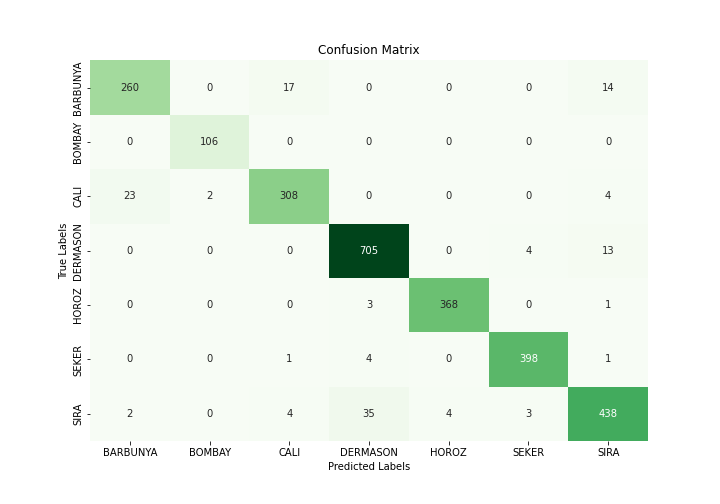
\includegraphics[scale=0.3]{../Plots/Classification tree confusion matrix.png}}
%     \caption{Classification tree confusion matrix}
%     \label{clf confusion matrix}
% \end{figure}

\end{document}